\documentclass[11pt,a4paper]{article}
\usepackage[top=3cm, bottom=2cm, left=3cm, right=2cm]{geometry}
\usepackage[utf8]{inputenc}
% \usepackage[T1]{fontenc}
\usepackage{amsmath, amsfonts, amssymb}
\usepackage{siunitx}
\usepackage[brazil]{babel}
\usepackage{graphicx}
\usepackage[margin=10pt,font={small, it},labelfont=bf, textfont=it]{caption}
\usepackage[dvipsnames, svgnames]{xcolor}
\DeclareCaptionFont{MediumOrchid}{\color[svgnames]{MediumOrchid}}
\usepackage[pdftex]{hyperref}
\usepackage{natbib}
\bibliographystyle{plainnat}
\bibpunct{[}{]}{,}{s}{}{}
\usepackage{color}
\usepackage{footnote}
\usepackage{setspace}
\usepackage{booktabs}
\usepackage{multirow}
\usepackage{subfigure}
\usepackage{fancyhdr}
\usepackage{leading}
\usepackage{indentfirst}
\usepackage{wrapfig}
\usepackage{mdframed}
\usepackage{etoolbox}
\usepackage[version=4]{mhchem}
\usepackage{enumitem}
\usepackage{caption}
\DeclareCaptionLabelFormat{figuras}{\textcolor{CarnationPink}{Figura \arabic{figure}}}
\captionsetup[figure]{labelformat=figuras}

\makeatletter
\renewcommand\tagform@[1]{\maketag@@@{\color{CarnationPink}(#1)}}
\makeatother

\renewcommand{\theequation}{Eq. \arabic{equation}}
\renewcommand{\thefigure}{Fig. \arabic{figure}}

\setlist[itemize]{label=\textcolor{CarnationPink}{$\mathbf{\square}$}}

\setlist[enumerate]{label=\textcolor{CarnationPink}{\arabic*.}, align=left}


\newcounter{exemplo}

\NewDocumentEnvironment{exemplo}{ O{} }{%
\allowbreak
\setlength{\parindent}{0pt}
  \begin{mdframed}[
  leftline=true,
  topline=false,
  rightline=false,
  bottomline=false,
  linewidth=2pt,
  linecolor=CarnationPink,
  frametitlerule=false,
  frametitlefont=\Large\bfseries\color{CarnationPink},
  frametitle={\color{CarnationPink}\normalfont\bfseries #1},
  ]
}{%
  \end{mdframed}
}

\setlength{\fboxsep}{10pt}
\setlength{\fboxrule}{1pt}
\usepackage{float}
\renewcommand{\thefootnote}{\alph{footnote}}
\usepackage{url}
\hypersetup{
    colorlinks=true,
    linkcolor=cyan,
    filecolor=cyan,      
    urlcolor=cyan,
    citecolor=cyan,
    pdftitle={Resumos}
}
\pagestyle{fancy}
\fancyhf{}
\renewcommand{\headrulewidth}{0pt}
\rfoot{Página \thepage}

\title{Dosimetria}
\author{Detectores de Radiação\nocite{*}}
\date{\textit{Dalila Mendonça}}
\begin{document}
	\maketitle

\section{Propriedades Gerais dos Detectores de Radiação}

    Um detector quando submetido à radiação, terá um volume que será responsável por detectar a radiação e efetuar a leitura. Quando a radiação interage com o volume do detector, ela irá causar ionizações, ou seja, arrancará um elétron do átomo inicialmente neutro, e fará com que seja formado um par elétron íon, cargas negativas e cargas positivas. A interação ou o total freamento da partícula ocorre em um tempo muito curto, o que permite dizer que a deposição de energia é feita instantaneamente. 

    Assumindo a interação devido a apenas um quanta de energia (uma única partícula), a carga gerada dentro do detector ocorrerá então no tempo $t = 0$ (instantâneo). Na sequência, a carga deverá ser coletada na forma de sinais elétricos, cujo processo de detecção normalmente está acompanhado de um campo elétrico interno, que faz com que as cargas positivas e negativas se movam em direções opostas. 

    O tempo para coletar todas as cargas formadas nos detectores varia de um tipo de detector para outro, por exemplo as câmaras de ionização o tempo para coletar todas as cargas é da ordem de poucos milissegundos, enquanto que o tempo de coleção dos  diodos semicondutores é da ordem de poucos nanossegundos. Esses tempos de coleta estão relacionados à mobilidade dos portadores de carga e também à distância que os portadores de carga percorrem até serem coletadas no eletrodo coletor.

    Portanto, para a interação de apenas um quanta de energia, a resposta do detector será uma corrente que flui por um tempo igual ao tempo de coleta da carga. A  \ref{fig:esquemaTempoColetaCorrente} mostra uma possível dependência temporal da corrente do detector, onde $t_c$ é o tempo para coletar a carga;

        \begin{figure}[h]
            \centering
            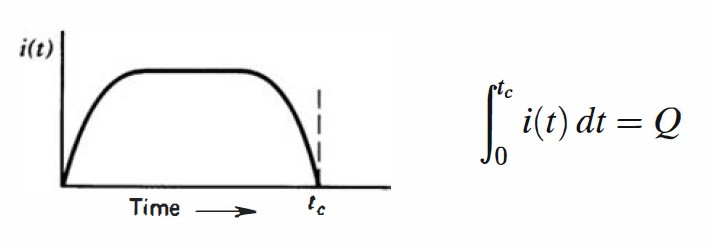
\includegraphics[width=0.7\textwidth]{Imagens/esquemaTempoColetaCorrente.jpg}
            \caption{Corrente em função do tempo de coleta da carga}
            \label{fig:esquemaTempoColetaCorrente}
        \end{figure}

	\noindent A integral da corrente ao longo de todo o tempo de coleta é igual quantidade total de carga gerada naquela interação específica. 

	Em situações reais, vários quantas estão interagindo com o volume do detector ao longo de um período de tempo. Portanto, para os casos em que há uma alta taxa de irradiação, a corrente gerada pode ser devida a mais de uma interação.  Assumindo que o detector está submetido a uma baixa taxa de radiação, de forma que cada interação irá gerar uma corrente que pode ser distinguida das demais interações. A medida que cada interação ocorre, serão gerados pulsos de correntes elétricas de modo que a intensidade de duração do pulso de corrente poderá variar dependendo do tipo de interação. A  \ref{fig:esquemaCorrentePulsada} mostra um esquema da corrente elétrica instantânea fluindo no detector ao longo do tempo.

		\begin{figure}[h]
			\centering
			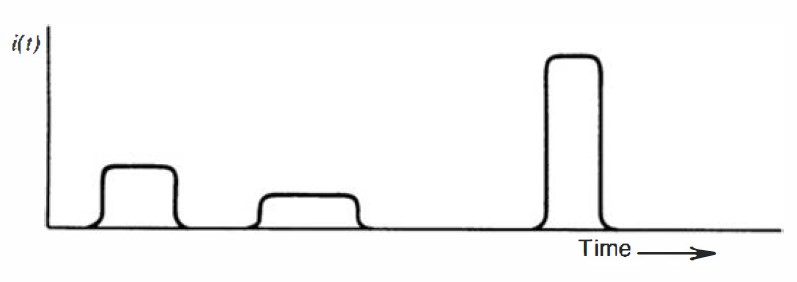
\includegraphics[width=0.7\textwidth]{Imagens/esquemaCorrentePulsada.jpg}
			\caption{Esquema de Pulsos de Corrente ao longo do tempo de medição do detector}
			\label{fig:esquemaCorrentePulsada}
		\end{figure}

	\noindent Pode-se observar diferentes intensidades de corrente e diferentes tempos de coleta de cada pulso. Nota-se também que, como a emissão de radiação é um processo aleatório, os intervalos de tempo entre um pulso de corrente e outro também é aleatoriamente distribuído. 
      
	\subsection{Modos de Operação Dos Detectores}

		Existem três modos de operação dos detectores, \textcolor{CarnationPink}{\textbf{\textit{Modo Pulso, Modo Corrente e Modo de tensão quadrada média (MSV)}}}; ambos operam de forma diferente e estão inter-relacionados através de suas dependências com as sequências de pulsos de correntes geradas no detector. 

		Como a energia depositada no detector é diretamente relacionada com a carga total $Q$ geradas através das interações dos quantas de energia com o detector, é de interesse que todas as cargas sejam coletadas e portanto o instrumento de medição irá operar no \textcolor{CarnationPink}{modo pulso} de forma que toda interação individual seja registrada. 

		O \textcolor{CarnationPink}{modo pulso} também é utilizado nos \textcolor{CarnationPink}{contadores de pulsos}, que se enquadra naquelas situações onde não é de interesse registrar a distribuição de energia da radiação, ou seja, não é de interesse obter energia depositada pelos quantas de radiação, o interesse é apenas obter a intensidade da radiação incidente; Para estes casos, é estabelecido um limiar de baixo nível para os pulsos gerados de forma qua qualquer pulso de corrente acima deste limiar é registrado pelo detector, independente do valor de Q.

		O \textcolor{CarnationPink}{modo corrente} e o \textcolor{CarnationPink}{modo MSV} são utilizados naquelas situações em que a taxa radiação é muito alta de forma que o modo pulso seja impraticável pois o tempo entre eventos adjacentes é muito pequeno de forma que não seja possível realizar uma análise adequada da carga coletada e os pulsos de corrente gerados podem se sobrepor ao longo do tempo; Sendo necessário, então, utilizar instrumentos de medição que respondem à media de tempo no qual ocorrem muitos eventos individuais;

		\subsubsection{Modo Corrente}

			A  \ref{fig:esquemaModoCorrente} apresenta o esquema de um detector operando no modo corrente, onde um amperímetro é conectado aos terminais de saída do detector de radiação;

				\begin{figure}[h]
					\centering
					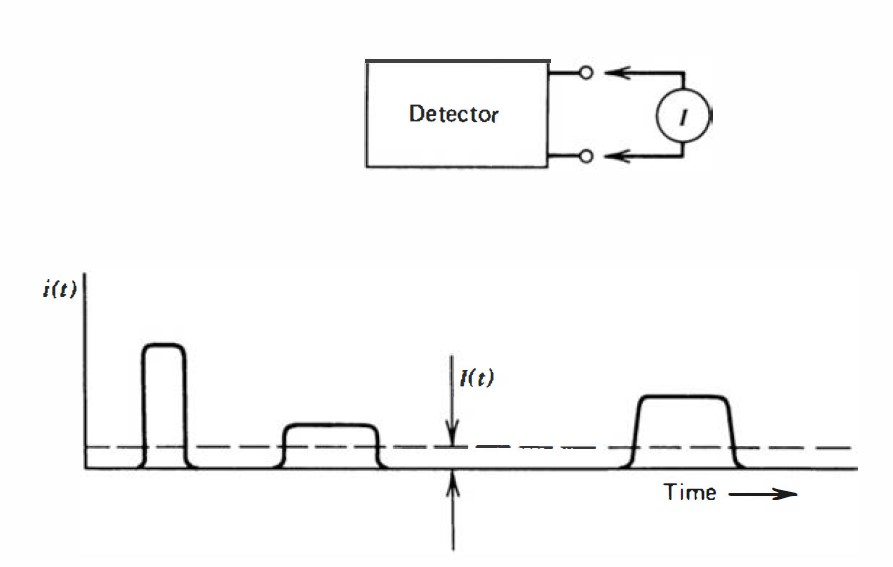
\includegraphics[width=0.7\textwidth]{Imagens/esquemaModoCorrente.jpg}
					\caption{Esquema de Detector Operando no Modo Corrente.}
					\label{fig:esquemaModoCorrente}
				\end{figure}
			
			No modo corrente, assume-se que o tempo de resposta T do detector é fixo, e portando diversos pulsos de corrente emitidos em um tempo t serão coletados ao longo do tempo de resposta do detector, gerando uma corrente dependente do tempo dada por:
			
				\begin{equation}
					I(t) = \frac{1}{T} \int_{t-T}^{t} i (t') \,dt' 
				\end{equation}

			\noindent Como o tempo de resposta T é muito maior que o intervalo de tempo entre os pulsos de corrente individuais, o efeito é compensar muitas das flutuações nos intervalos entre as interações individuais e registrar uma corrente média que depende do produto da taxa de interação e a carga média por interação.

			A corrente média é dada pelo produto da taxa de eventos com a média de carga produzida por cada evento; portanto:

				\begin{equation}
					I_0 = rQ = r\frac{E}{W}q
				\end{equation}
			
			\noindent onde:

				\begin{tabular}{l l l }
				r & = & Taxa de Eventos \\
				Q & = & carga produzida por cada evento \\
				E & = & energia média depositada por cada evento \\
				W & = & Energia média para produzir um par elétron-íon \\
				q & = & carga elétrica ($1.6 \times 10^{-19}C$)
				\end{tabular}

			Para uma irradiação estacionária do detector, a corrente média pode ser descrita como a soma da corrente constante $I_0$ com a componente de flutuação da corrente dependente do tempo ($\sigma_i(t)$), no qual é a variável aleatória dependente do tempo que ocorre como consequência da natureza aleatória dos eventos interagindo com o detector,  como mostra a  \ref{fig:esquemaCorrenteFlutuacao}.

			\begin{figure}[h]
				\centering
				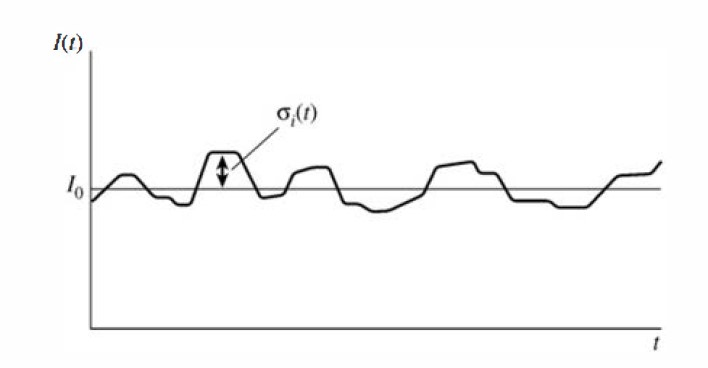
\includegraphics[width=0.7\textwidth]{Imagens/esquemaCorrenteFlutuação.jpg}
				\caption{Irradiação estacionária com flutuação}
				\label{fig:esquemaCorrenteFlutuacao}
			\end{figure}

		\subsubsection{Modo Pulso}

			A natureza do sinal produzido por um único evento depende das características de entrada do circuito no qual o detector está conectado, normalmente utilizando um pré-amplificador. A  \ref{fig:esquemaModoPulso} apresenta um esquema básico de um circuito utilizado no modo pulso. 

				\begin{figure}[h]
					\centering
					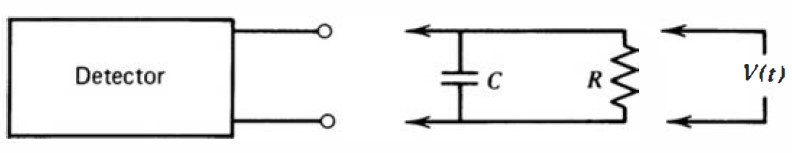
\includegraphics[width=0.8\textwidth]{Imagens/esquemaModoPulso.jpg}
					\caption{Circuitos de um detector operando em modo pulso}
					\label{fig:esquemaModoPulso}
				\end{figure}

			\noindent Onde R representa a resistência de entrada do circuito e C representa a capacitância equivalente que considera a capacitância do detector e do circuito de medição; Caso um pré-amplificador seja acoplado ao detector, então R será a resistência de entrada e C será a soma das capacitâncias do detector, do cabo que conecta o detector ao pré-amplificador e capacitância de entrada do próprio pré-amplificador. $V(t)$ é a tensão dependente do tempo, com o qual o modo pulso é baseado. 

			Resistência elétrica é a oposição que um material apresenta à passagem de corrente elétrica através dele. Essa oposição é causada pelos elétrons que compõem o material e que se movem em resposta a um campo elétrico aplicado, colidindo com outras partículas do material e transferindo energia para elas. 

			A resistência elétrica limita a quantidade de corrente elétrica que pode fluir através do circuito. A Lei de Ohm estabelece que a corrente elétrica que flui através de um material é diretamente proporcional à diferença de potencial elétrico aplicada (tensão) e inversamente proporcional à resistência elétrica do material, ou seja:

				\begin{equation}
					I = \frac{V}{R}
				\end{equation}

			\noindent Onde I é a corrente elétrica dada em amperes (A), V é a diferença de potencial dada em volts (V) e R é a resistência dada em ohms ($\omega$).

			A Capacitância é uma grandeza elétrica que mede a capacidade de um objeto de armazenar carga elétrica quando submetido a uma diferença de potencial elétrico e está envolvida em circuitos elétricos que possuem capacitores.
			
			Os capacitores são dispositivos eletrônicos que consistem em duas placas condutoras separadas por um material isolante (dielétrico). Quando uma tensão é aplicada ao capacitor, as cargas elétricas se acumulam nas placas, criando um campo elétrico entre elas. Esse campo elétrico é proporcional à carga elétrica armazenada no capacitor e inversamente proporcional à capacitância do capacitor.

			A capacitância é dada pela relação entre a carga elétrica armazenada e a diferença de potencial elétrico aplicada ao capacitor, dada por:

				\begin{equation}
					C = \frac{Q}{V}
				\end{equation}

			\noindent Onde C é a capacitância em farads (F), Q é a carga elétrica armazenada em coulombs (C) e V é a diferença de potencial elétrico (tensão) em volts (V) aplicada ao capacitor.
			
			Um circuito RC é um circuito elétrico composto por um resistor (R) e um capacitor (C) conectados em série ou em paralelo. A operação desse circuito depende da capacidade do capacitor de armazenar e liberar carga elétrica.

			Quando uma tensão é aplicada ao circuito, o capacitor começa a carregar. Durante esse processo, a corrente elétrica flui através do resistor, reduzindo a tensão aplicada ao capacitor. A taxa de carga depende do valor da resistência e da capacitância do circuito, conforme determinado pela constante de tempo.

			A constante de tempo em um circuito RC é um parâmetro que indica a rapidez com que um capacitor carrega ou descarrega em resposta a uma mudança na tensão aplicada a ele através de um resistor. É uma medida do tempo necessário para que a tensão do capacitor atinja aproximadamente 63,2\% do seu valor final após uma mudança na tensão de entrada.

			Após um certo tempo, o capacitor atinge seu limite de carga máxima e começa a armazenar energia elétrica. Se a tensão aplicada ao circuito for interrompida, o capacitor começa a descarregar através do resistor, liberando a energia armazenada. A taxa de descarga também depende do valor da resistência e da capacitância, conforme determinado pela constante de tempo.
			
			A constante de tempo para um circuito RC  é dada por:
			
				\begin{equation}
					\tau = R \cdot C
				\end{equation}

			\noindent onde $\tau$ é a constante de tempo em segundos, R é a resistência em ohms e C é a capacitância em farads. 
			
			A constante de tempo é importante em circuitos que envolvem a carga e descarga de capacitores, pois ela afeta a taxa de mudança da tensão no capacitor e, portanto, o comportamento do circuito como um todo.
			
			Pode-se então avaliar dois extremos de operação: Quando a constante de tempo do circuito é muito menor que o tempo para a coleta da carga e quando a constante de tempo é muito maior que o tempo para a coleta da carga.

			\begin{wrapfigure}{r}{0.5\textwidth}
				\centering
				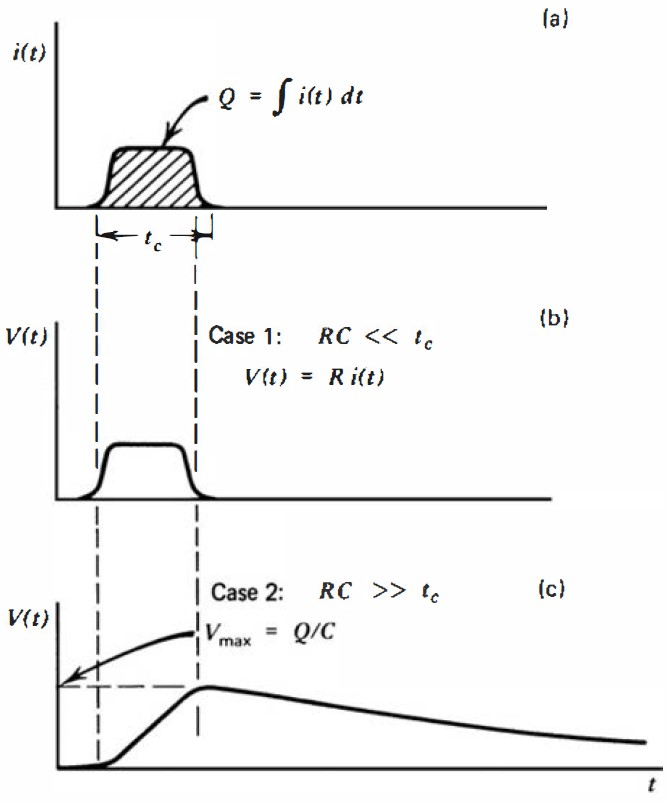
\includegraphics[width=0.41\textwidth]{Imagens/esquemaCorrentesCircuitoRC.jpg}
				\caption{Extremos de Operação}
				\label{fig:esquemaCorrenteCircuitoRC}
			\end{wrapfigure}


			$\tau \ll t_c$: Neste caso a constante de tempo do circuito externo é mantida pequena comparada ao tempo para coleta da carga, de forma que a corrente fluindo através da resistência R é essencialmente igual ao valor instantâneo da corrente fluindo no detector. O sinal da voltagem V(t) produzidos sob estas condições tem a forma aproximadamente idêntica à dependência temporal da corrente produzida dentro do detector, como mostra a  \ref{fig:esquemaCorrenteCircuitoRC}(b). Os detectores de radiação as vezes operam sob estas condições quando informações a respeito de altas taxas de eventos ou informações temporais são mais importantes que uma informação precisa da energia.

			$\tau \gg t_c$: Este é o principal modo de operação dos detectores que operam no modo pulso. Neste caso a constante de tempo é mantida grande o suficiente quando comparada ao tempo de coleta da carga de modo que uma corrente muito pequena irá fluir através da resistência R durante o tempo de coleta da carga e a corrente do detector é momentaneamente integrada à capacitância. Se assumirmos que o tempo entre os pulsos é suficientemente grande, o capacitor começará a descarregar através da resistência, retornando a voltagem da resistência para zero, como mostra a  \ref{fig:esquemaCorrenteCircuitoRC} (c).


			\begin{itemize}
				\item O tempo necessário para o pulso do sinal alcançar seu valor máximo é determinado pelo tempo de coleção de carga dentro do próprio detector;
				\item O tempo necessário para restaurar a tensão do sinal para zero é determinado apenas pela constante de tempo do circuito elétrico.
				\item A amplitude do pulso de sinal é determinada pela seguinte relação:
					\begin{equation}
						V_{max} = \frac{Q}{C}
					\end{equation}
			\end{itemize}

			Portanto, o output de um detector operando em modo pulso consiste em uma sequência de pulsos de sinais individuais representando o resultado da interação de uma única partícula com o detector, e a amplitude de cada pulso individual reflete a quantidade de carga liberada nessa interação.

			Só existe uma proporcionalidade entre $V_{max}$ e a Carga $Q$ caso a capacitância se mantenha constante. Na maior parte dos detectores, a capacitância inerente é dada pela a forma e tamanho do capacitor utilizado no circuito de forma que é garantida uma capacitância constante. Em outros casos, como ocorre com os diodos semi-condutores, a capacitância pode mudar devido a uma variação nos parâmetros normais de operação. Nestes casos, pulsos de voltagem com diferentes amplitudes podem ser gerados a partir da mesma carga total liberada na interação Q. 

			Comparando os detectores operando em modo pulso com os detectores operando em modo corrente, podemos inferir que:

			\begin{itemize}
				\item A sensibilidade alcançada dos detectores operando no modo pulso é frequentemente muito maior que a sensibilidade dos detectores que operam no modo corrente, pois cada interação individual pode ser detectada como um pulso distinto.
				\item No modo pulso, os limiares de detecção são definidos a partir dos níveis de radiação de fundo; No modo corrente, a corrente mínima detectável pode representar uma taxa média de eventos muito maior que a radiação de fundo;
				\item No modo pulso, cara amplitude de pulso carrega alguma informação que é sempre útil ou uma parte necessária de uma aplicação em particular; Já no modo corrente, a informação a respeito da amplitude do pulso é perdida e todas as interações, independente da amplitude, contribuem para a corrente média medida. 
			\end{itemize}

	\subsection{Espectro de Altura de Pulso}

		Quando um detector opera no modo pulso, cada amplitude de pulso gerada carrega informação a cerca da carga gerada em cada interação; Porém, ao avaliar diversos pulsos, nota-se que as amplitudes nem sempre são as mesmas e isto se deve à diferenças de energias das partículas incidentes ou até mesmo flutuações inerentes à resposta do detector em feixes monoenergéticos. 

		A distribuição de amplitude de pulso pode ser utilizada para deduzir informações a respeito da radiação incidente ou para obter informações a respeito da operação do próprio detector. Estas distribuições podem ser exibidas na forma integral ou diferencial.



		\subsubsection*{Distribuição Diferencial de Altura de Pulso}

			A  \ref{fig:distribuicaoDeAlturaDePulso} (a) fornece uma distribuição hipotética onde: a abscissa é a escala linear de amplitude de pulso que vai de zero até o maior valor de amplitude observado para a fonte, fornecida em volts (V); O eixo das ordenadas representa o número diferencial $dN$  de pulsos observados para uma amplitude dentro de um incremento diferencial de amplitude $dH$, dividido por esse incremento, ou seja $dN/dH$, fornecido em \unit{V^{-1}}.

			O número de pulsos cuja amplitude está entre dois valores pré-determinados $H_1$ e $H_2$ podem ser obtidos através da área da curva limitada por estas duas amplitudes, ou seja:

				\begin{equation}
					N_{H_1 \rightarrow  H_2} = \int_{H_1}^{H_2} \frac{dN}{dH}  \,dH 
				\end{equation}

				\begin{wrapfigure}{l}{0.6\textwidth}
					\centering
					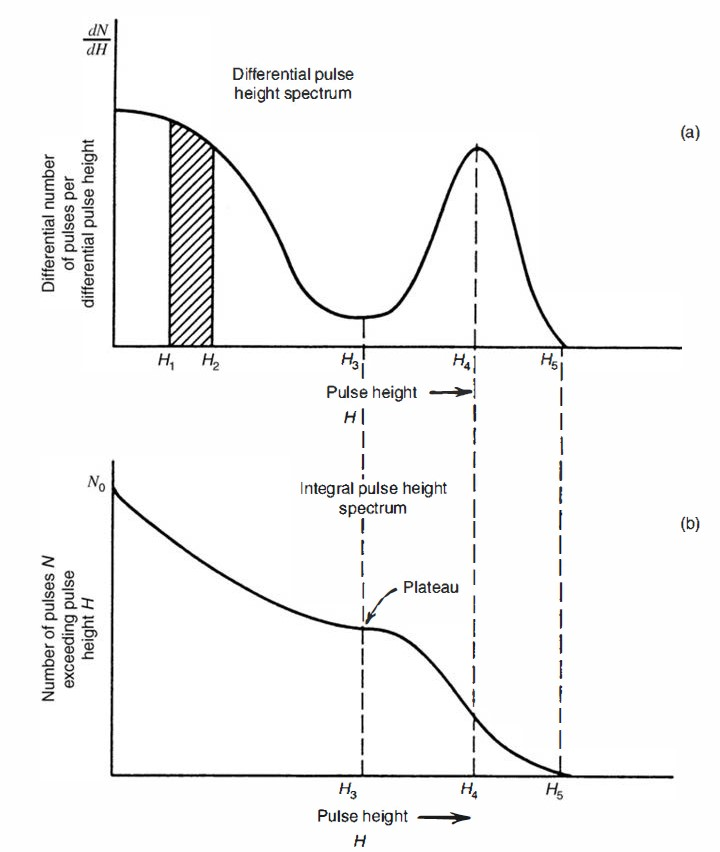
\includegraphics[width=0.59\textwidth]{Imagens/distribuicaoDeAlturaDePulso.jpg}
					\caption{Distribuições de Amplitude}
					\label{fig:distribuicaoDeAlturaDePulso}
				\end{wrapfigure}

			O número total de pulsos $N_0$ pode ser obtido através da área total embaixo da curva, ou seja:

				\begin{equation}
					N_0 = \int_{0}^{\infty} \frac{dN}{dH} \,dH
				\end{equation}

			A amplitude de pulso máxima observada ($H_5$) é o ponto ao longo da abscissa no qual a distribuição vai para zero; Picos na distribuição, como ocorre em $H_4$, indicam que são encontrados uma grande quantidade de pulsos para aquela amplitude de pulso; Os vales na distribuição, como ocorre em $H_3$, indicam que são encontrados poucos números de pulsos para aquela determinada amplitude de pulso. 

		\subsubsection*{Distribuição Diferencial de Altura de Pulso}

			A  \ref{fig:distribuicaoDeAlturaDePulso} (b) mostra a distribuição integral para o mesmo espectro apresentado na  \ref{fig:distribuicaoDeAlturaDePulso} (a). O eixo das abscissas também representa a escala de amplitude de pulso, e o eixo das ordenadas apresenta o número de pulsos N no qual a amplitude excede o valor apresentado no eixo das abscissas H. N diminui em função H pois cada vez menos pulsos estarão acima de uma amplitude $H_i$ que pode aumentar seu valor além de zero. 
			
			Como todos os pulsos possuem uma amplitude finita maior que zero, então $H = 0$ representa o número total de pulsos observados $N_0$ e a medida que H aumenta a N diminui até que a distribuição integral cai para zero na amplitude de pulso máxima observada ($H_5$). 


		A amplitude da distribuição diferencial, ou seja, o número de pulsos de qualquer amplitude de pulso H é dada pelo valor absoluto da curva da distribuição integral no mesmo valor H; Nos locais onde aparecem picos na distribuição diferencial, representam pontos de máximo local na distribuição integra; E semelhantemente, as regiões de vale na distribuição diferencial representa os mínimos locais de amplitudes de pulsos na distribuição integral. 


	\subsection{Curvas de Contagem e Platôs}

		Quando os detectores operam no modo de contagem pulsada, os pulsos do detector são enviados para um dispositivo de contagem que possui um nível fixo de discriminação, ou seja possui um limiar de amplitude de pulso. Para que um pulso de sinal seja registrado pelo circuito do contador este pulso deverá exceder um limiar de amplitude de pulso $H_d$. É possível variar o limiar $H_d$ durante a medição afim de se obter informações a cerca da distribuição de amplitudes de pulso, e medidas realizadas com estas variações resultará da distribuição integral de amplitudes de pulso. 

		Ao realizar uma medida de contagem, a medição deverá ser conda de modo que se estabeleça um ponto de operação no qual irá ser alcançada a maior estabilidade sob longos períodos de tempo. Ou seja, durante uma medição podem ocorrer pequenos desvios em $H_d$ e portanto deve ser estabelecido um ponto de operação que fará com que esse desvio tenha influência mínima na contagem medida. Como mostra a  \ref{fig:distribuicaoDeAlturaDePulso}, o ponto em $H_3$ se con como um ponto estável de operação; Este ponto representa o ponto de mínimo global da distribuição diferencial de forma que representa um ponto com  variação mínima na curva integral, portanto pequenos desvios no limiar $H_d$ terão um impacto mínimo no número total de pulsos registrados. No geral, regiões de mínimo na curva integral são chamados de platô de contagem e representam áreas de operação no qual é possível alcançar uma sensibilidade mínima a variações no limiar de amplitude. 

		O platô em contagem de dados também é observado em processos no qual a carga produzida a cada interação é aumentada para um determinado detector de radiação; onde muitas vezes é possível variar o ganho ou a amplificação fornecida para a carga produzida na interação. Esta variação pode ser feita alterando o fator de amplificação de um amplificador linear posicionado entre o detector e o circuito de contagem, ou pode ser feita diretamente alterando a voltagem aplicada no próprio detector. 

		A  \ref{fig:curvaContagemGanho} (a) apresenta uma distribuição diferencial de amplitude de pulso, para três valores diferentes de ganho da voltagem. Neste caso, o valor do ganho (G) pode ser definido como a razão entre a amplitude da voltagem para um dado evento no detector e a mesma amplitude antes de algum parâmetro ser alterado, como o fator de amplificação ou a voltagem do detector. 

			\begin{figure}[h]
				\centering
				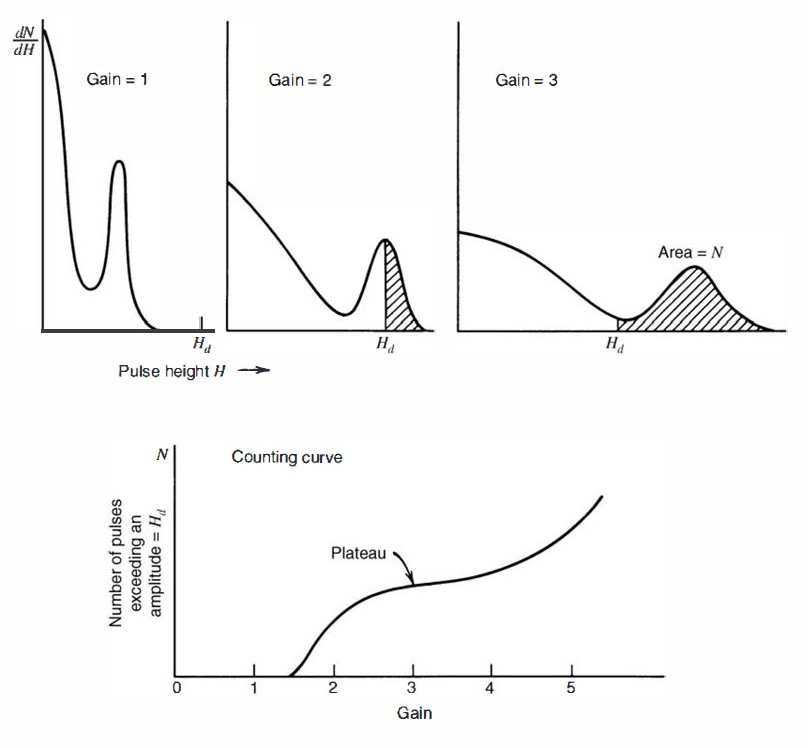
\includegraphics[width=0.8\textwidth]{Imagens/curvaContagemGanho.jpg}
				\caption{Exemplo de uma curva de contagem gerada através da variação do ganho mantendo as condições da fonte constante}
				\label{fig:curvaContagemGanho}
			\end{figure}

		
		Ao manter a irradiação constante, quanto maior o ganho na voltagem maior será a amplitude de pulso máxima, porém em ambos os casos a área sob a curva diferencial se manterá constante, ou seja, o número total de pulsos  será sempre o mesmo. A  \ref{fig:curvaContagemGanho} mostra que para o ganho G = 1, nenhuma contagem será registrada pois todas as amplitudes de pulso estão abaixo do limiar de amplitude para detecção. Ao realizar contagens em função do ganho da voltagem, obtem-se a distribuição integral, chamada de curva de contagens, apresentada na  \ref{fig:curvaContagemGanho} (b). Devido à pequenos valores de ganho, nenhum pulso é contado, porem a medida que o ganho é aumentado, aumenta-se o número de pulsos contados até que o ganho seja suficiente para contar todos os pulsos. 

		O platô na curva de contagem pode ser previsto com base no valor de ganho que faz com que o limiar de amplitude $H_d$ coincida aproximadamente com um ponto de mínimo na curva diferencial. 


	\subsection{Resolução de Energia}

		Diversas aplicações de detectores de radiação tem como objetivo medir a distribuição de energia da radiação incidente, chamado de forma geral como espectroscopia da radiação. A  \ref{fig:funcoesDeResposta} ilustra a distribuição diferencial de amplitude de pulso produzida por um detector submetido a um feixe monoenergético; Esta distribuição é chamada de \textbf{função resposta} de um detector para a energia utilizada na sua determinação. A curva chamada de ``Boa Resolução'' ilustra uma possível distribuição em torno da amplitude média de pulso $H_0$; A curva chamada de ``Baixa Resolução'', ilustra a resposta de um detector com um desempenho inferior. Desde que ambos os casos registrem o mesmo número de pulsos, as áreas embaixo das curvas são iguais.

		\begin{figure}[h]
			\centering
			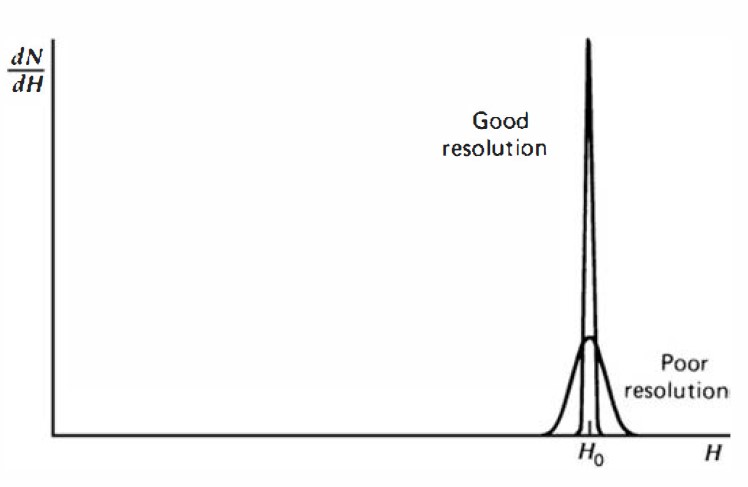
\includegraphics[width=0.7\textwidth]{Imagens/funcoesDeResposta.jpg}
			\caption{Funções de Resposta}
			\label{fig:funcoesDeResposta}
		\end{figure}

		Embora ambas as distribuições estejam centradas em torno do valor médio $H_0$, a largura da distribuição para a baixa resolução é muito maior. Esta largura reflete o fato de que foi registrada uma grande quantidade de flutuação de pulso a pulso embora a mesma energia tenha sido depositada para cada evento. Se a quantidade destas flutuações é for cada vez menor, a largura da distribuição será cada vez menor e a forma da curva se aproximará para uma função delta de dirac. 

		A definição para a resolução de energia de um detector pode ser observada na  \ref{fig:resolucaoDeEnergia}, onde a distribuição diferencial de amplitude de pulso é determinada para um detector submetido a um feixe monoenergético. 

			\begin{figure}[h]
				\centering
				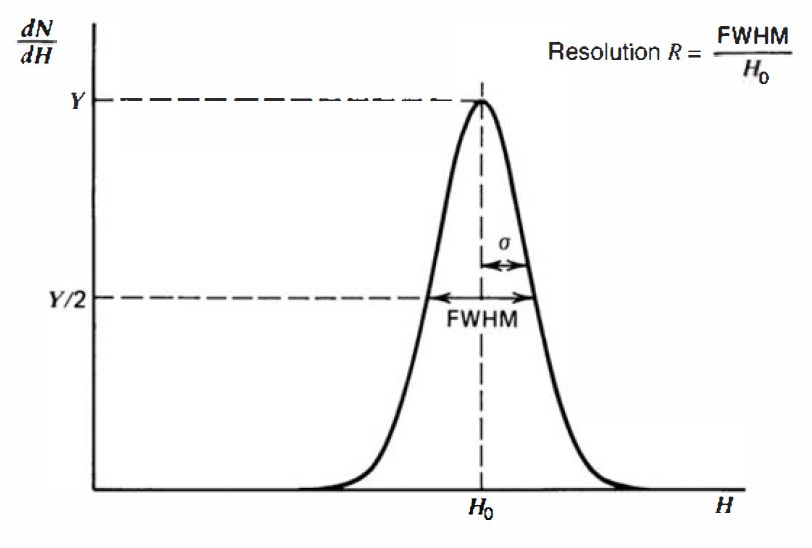
\includegraphics[width=0.7\textwidth]{Imagens/resolucaoDeEnergia.jpg}
				\caption{Resolução de Energia}
				\label{fig:resolucaoDeEnergia}
			\end{figure}


		A largura à meia altura (FWHM,  do inglês \textit{Full Width at Half Maximum}) é definida como a largura da distribuição na metade da altura do pico relacionado a $H_0$. Esta definição assume que qualquer sinal de fundo ou qualquer sinal contínuo que possa sobrepor o pico é negligenciável ou foi subtraído do sinal do pico. A resolução R é uma grandeza adimensional, e  sua fração é convencionalmente expressa em percentual. Um diodo possui resolução energética de aproximadamente 1\% enquanto que detectores cintiladores possuem uma resolução energética variando entre ~3\% até ~ 10\%.

		Quanto menor o valor para a resolução de energia, melhor será a habilidade do detector distinguir duas radiações cujas energias estão próximas uma da outra. Uma regra prática é que o detector deve ser capaz de detectar duas energias separadas por mais de uma FWHW .

		Alguns fatores que causam flutuações na resposta de um detector são: desvios nas características de operação do detector durante a medição; fontes de ruídos aleatórias dentro do detector e do sistema de instrumentação e o ruído estatístico proveniente da natureza discreta do próprio sinal medido. 
		
		O ruído estatístico representa a quantidade mínima de flutuação que não pode pode ser removida independente da qualidade do sistema de medição utilizado. O ruído estatístico surge devido ao fato de que a carga Q gerada dentro do detector devido a um quanta de radiação  não é uma variável contínua, mas sim um valor discreto do número de portadores de carga. Pode ser feita uma estimativa da flutuação inerente da detecção assumindo que os portadores de carga criados se se aproximam de distribuição Gaussiana.

	\subsection{Eficiência de Detecção}

		A eficiência de detecção varia com o tipo de radiação para o qual o detector será utilizado, sendo diferente para radiações diretamente ionizantes e indiretamente ionizantes.

		Quando uma radiação diretamente ionizante, como as partículas alfa e os elétrons, entra na cavidade do detector, causarão imediatamente ionizações e excitações no volume da cavidade, e após viajar uma pequena fração do seu alcance será liberado pares de íons suficientes que farão com que o pulso resultante seja grande o suficiente para ser registrado; Portanto, garantindo que o detector consiga detectar toda partícula carregada que entra em sua cavidade, pode-se dizer que o detector possuirá uma eficiência de contagem de 100\%. 

		Enquanto que a radiação diretamente ionizante é imediatamente detectada entrar na cavidade do detector, para detectar uma radiação indiretamente ionizante, ela deve primeiramente sofrer uma interação significante no detector, para então ser possível detectá-la. Como estas radiações podem viajar largas distâncias entre as interações, alguns quantas dessa radiação não serão detectados e portanto a eficiência do detector será sempre menor que 100\%.

		A eficiência na contagem é dividida entre:

			\begin{itemize}
				\item Eficiência Absoluta ($\epsilon_{abs}$), que é definida como a razão entre o número de pulsos registados $N_P$ e o número de partículas $N$ emitidas pela fonte, ou seja
				
					\begin{equation}
						\epsilon_{abs} = \frac{N_P}{N}
					\end{equation}
				
				A eficiência absoluta depende das propriedades do detector e da geometria  utilizada na contagem, sendo a principal componente a distância da fonte ao detector.
				
				\item Eficiência Intrínseca ($\epsilon_{int}$), que é definida como a razão entre o número de pulsos registrados $N_P$ e o Número de partículas $N_{in}$ que incidem no detector, ou seja:
				
					\begin{equation}
						\epsilon_{int} = \frac{N_P}{N_{in}}
					\end{equation}

				A eficiência intrínseca depende principalmente do material do detector, da energia da radiação, e da espessura de material do detector na região de incidência do feixe. 
			\end{itemize}

		A relação entre as eficiências para uma fonte isotrópica é dada por:

			\begin{equation}
					\epsilon_{int} = \epsilon_{abs} \cdot \left(\frac{4 \pi}{\Omega}\right)
			\end{equation}

		\noindent onde $\Omega$ é o ângulo sólido do detector visto a partir da posição da fonte.

	\subsection{Tempo Morto}

		Praticamente todos os detectores necessitam de uma quantidade de tempo mínima entre dois eventos para que ele possa registrar separadamente os dois pulsos, e essa limitação pode estar relacionada com a forma em si de realizar a detecção ou devido aos componentes eletrônicos do detector. Devido a natureza aleatória do decaimento radioativo, sempre existirá a possibilidade de um sinal verdadeiro não ser registrado por ocorrer muito próximo a outro evento. 

	\section{Detectores a Gás}

		\begin{figure}[h]
			\centering
			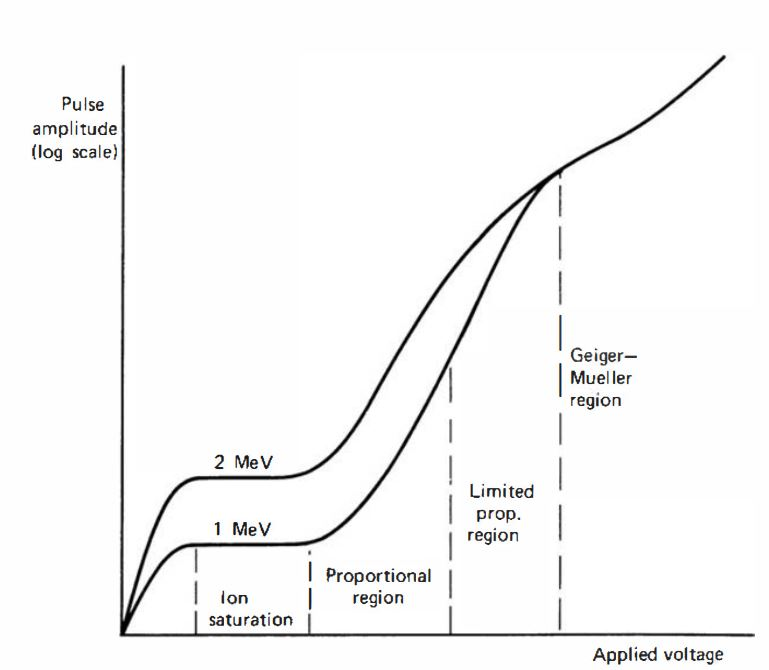
\includegraphics[width=0.7\textwidth]{Imagens/graficoDetectoresAGas.JPG}
			\caption{Regiões de Operação dos Detectores a gás}
			\label{fig:graficoDetectoresAGas}
		\end{figure}
	

	\subsection{Câmaras de Ionização}

		Considere duas placas separadas por uma cavidade de ar com uma diferença de potencial entre elas; Caso um fóton atravesse entre as placas, esse fóton pode interagir com o nitrogênio presente no ar quebrando a molécula formando um par de elétron e ion de nitrogênio. O elétron irá se mover na direção da placa positiva enquanto que o íon de nitrogênio irá se mover na direção da placa negativa. Haverá então uma diferença de carga líquida que pode ser medida em um eletrômetro. Caso milhares de fótons atravessem o meio, a quantidade de fótons que atravessam esse meio pode ser medida através da diferença da carga dividida pela massa de ar dentro das placas. Algumas das ionizações que acontecem enviarão elétrons para fora das placas, mas algumas dessas ionizações acontecerão fora das placas e enviarão íons dentro da região das placas. A medida que a quantidade de íons que se move para fora da região é igual a quantidade de íons que entram dentro da região, ocorre o equilíbrio eletrônico. Quando a condição de equilíbrio eletrônico é alcançada estará medindo o kerma no ar, caso contrário não estará medindo o Kerma precisamente

		\begin{figure}[h]
			\centering
			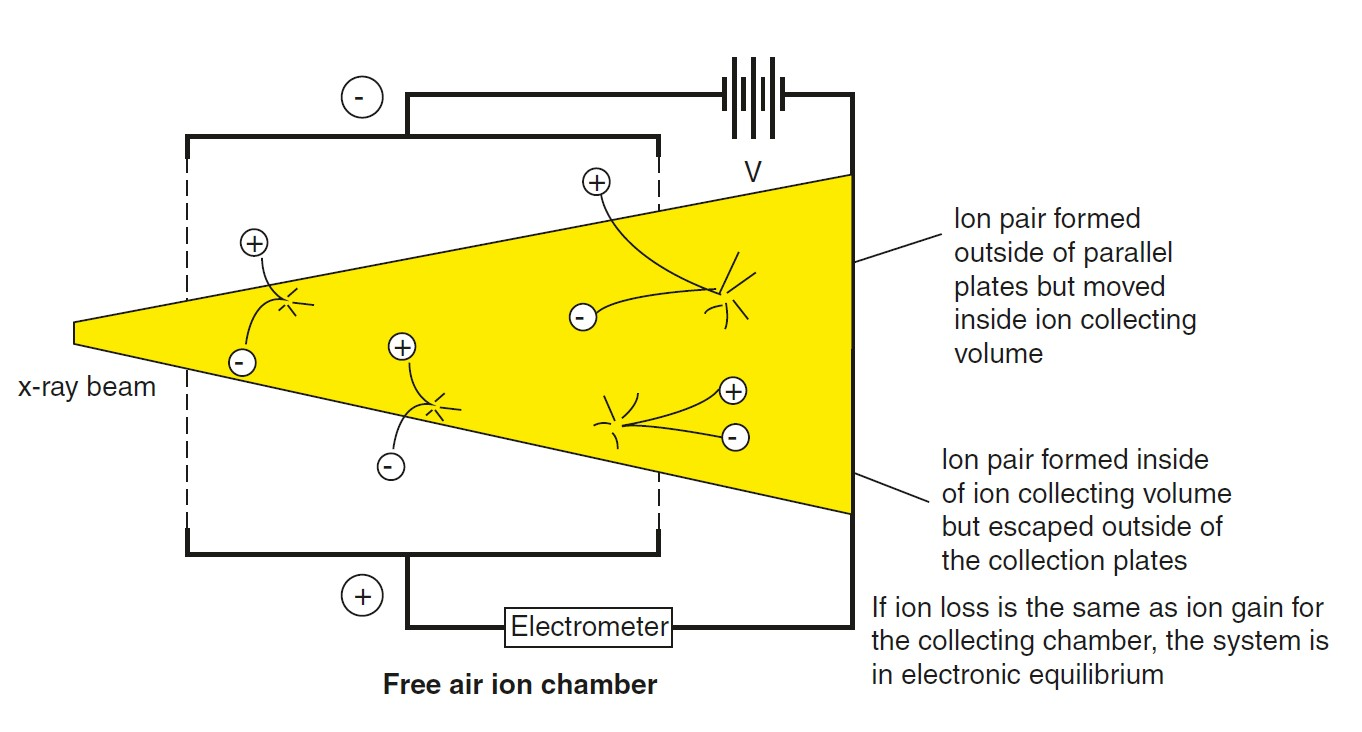
\includegraphics[width=0.5\textwidth]{Imagens/camaraArLivre.jpg}
			\caption{Câmara de Ar Livre}
			\label{fig:camaraArLivre}
		\end{figure}

	\subsection{Câmaras de Ar Livre}
		
		O padrão ouro para medida da radiação ionizante é a câmara de ionização de ar livre, porém sua conção requer tamanhos proporcionais ao alcance do elétron no ar, o que é muito grande para feixes de megavoltagem. Adicionalmente, uma vez que o meio é o ar livre sua conção é muito sensível à variações de temperatura, pressão, umidade e do campo elétrico. Por essas razões, as câmaras de ionização de ar livre só existem em laboratórios padrão. 

	\subsection{Câmaras do Tipo Dedal}

		Para obter uma câmara de ionização mais compacta (comparado à câmara de ar livre), é necessário utilizar um eletrodo central e uma parede externa;  O número de elétrons entrando na cavidade deve ser o mesmo número de elétrons saindo da cavidade a fim de alcançar o equilíbrio eletrônico, e isto normalmente irá requerer uma cavidade de ar muito larga;
		
		Porém, esta condição pode ser respeitada se as paredes que circundam a cavidade de ar forem feitas com um material muito mais denso mas ainda ter um número atômico semelhante ao número atômico das moléculas de ar; Com uma parede ``equivalente a ar denso'' em volta da cavidade de ar, a câmara pode ser feita pequena o suficiente para ser utilizada clinicamente.

		Caso a câmara seja pequena o suficiente de modo que ao ser inserida em um material a distribuição dos elétrons não seja alterada devido a presença da câmara, então a teoria cavitária de Braag-Gray pode ser utilizada para calcular a dose nessa região (Fig. \ref{fig:camaraDedal}.). 

		A Exposição para uma câmara dedal é calculada a partir da seguinte equação:
			\begin{equation}
				X = \frac{Q}{\rho \times \nu} \times \frac{1}{A}
			\end{equation}

		\begin{exemplo}[Onde]
			\begin{itemize}[label=\textcolor{CarnationPink}{$\star$}]
				\item $\mathbf{X}$ é a exposição;
				\item $\mathbf{Q}$ é a carga medida pelo eletrômetro;
				\item $\mathbf{\rho}$ é a densidade do ar;
				\item $\mathbf{\nu}$ é o volume de ar;
				\item $\mathbf{A}$ é o fator de correção para considerar a perturbação da câmara no meio (pouco menor que 1.00).
			\end{itemize}
		\end{exemplo}

		\begin{figure}[h]
			\centering
			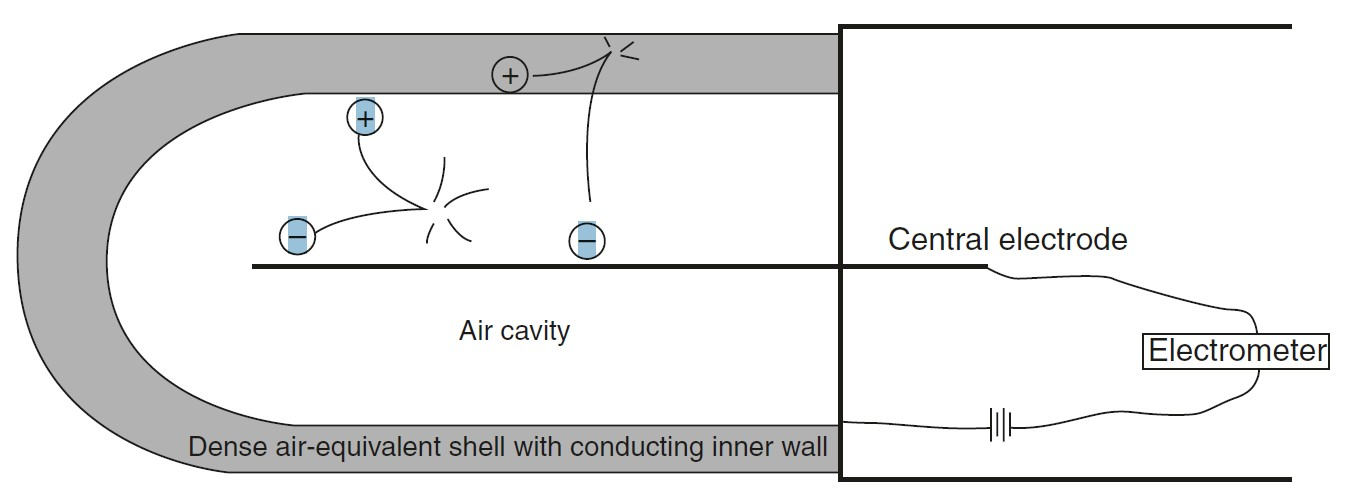
\includegraphics[width=0.5\textwidth]{Imagens/camaraDedal.jpg}
			\caption{Câmara dedal: constituída de um eletrodo central e uma parede condutora que pode ser utilizada para medir a carga. A parede feita de um material equivalente aos ar denso permite que a câmara tenha seu tamanho significativamente reduzido enquanto continua mantendo as condições de equilíbrio eletrônico e portanto medições precisas.}
			\label{fig:camaraDedal}
		\end{figure}

		Como a câmara do tipo dedal ainda continua sendo preenchida com ar, a densidade do ar dentro da cavidade ainda continuará sensível a variações de temperatura e pressão e portanto esses fatores devem ser considerados para a correção das leituras medidas.


	\subsection{Câmaras Condensadoras}

		As câmaras condensadoras operam como capacitores e mede a queda na voltagem na presença da radiação com um fator de conversão conhecido para a queda de voltagem por roetgen de exposição. Esta câmara é sensível a fótons com energias até $\sim$ 2 MeV e são insensíveis a altas energias devido aos elétrons que saltam da haste de metal ou do material do isolante. Esses tipos de detectores não são mais utilizadas em radioterapia. 

	\subsection{Câmaras tipo Farmer}
		
		As câmaras de ionização tipo farmer são as mais utilizadas em rotinas de radioterapia. Ela consiste em uma câmara cilíndrica com uma pequena cavidade central e é preenchida com um gás ou uma mistura de gases ionizantes. Esta é uma câmara relativamente estável e confiável para ser utilizadas na dosimetria de fótons de todas as energias nas faixas terapêuticas; A parede do volume sensível é feita de grafite puro e o eletrodo central é feito de alumínio ou grafite. Esta câmara de ionização possui um eletrodo de guarda para evitar corrente de fuga do eletrodo coletor e para definir o volume sensível mais consistentemente.

		A câmara de ionização tipo Farmer tem algumas características que a distingue das demais câmaras de ionização cilíndricas:

		\begin{itemize}[label=\textcolor{CarnationPink}{$\blacktriangleright$}]
			\item Além dos eletrodos coletores de íons e elétrons, a câmara de ionização tipo Farmer possui um eletrodo de referência. Esse eletrodo é geralmente um cilindro oco no centro da câmara, que ajuda a fornecer uma referência de potencial constante durante as medições.
			\item A geometria cilíndrica da câmara de ionização tipo Farmer é otimizada para garantir uma resposta de dose uniforme e uma boa representação da dose absorvida em tecidos. O tamanho da câmara também é projetado para ser adequado para uso em feixes de radiação.
		\end{itemize}

	\section{Dosímetros Termoluminescentes (TLD)}

		Os dosímetros TLD (Termoluminescent Dosimeters) são dispositivos utilizados para medir a dose de radiação ionizante. Eles são amplamente usados em aplicações de monitoramento de radiação, como proteção radiológica, controle de qualidade em radioterapia e monitoramento de exposição ocupacional.

		O funcionamento dos dosímetros TLD baseia-se no fenômeno da termoluminescência que é explicado pela teoria de bandas. A teoria de bandas descreve a estrutura eletrônica dos materiais sólidos em termos das energias permitidas para os elétrons e as bandas de energia disponíveis para eles.

		De acordo com a teoria de bandas, os átomos em um sólido formam uma estrutura cristalina que influencia a distribuição das energias dos elétrons. A estrutura cristalina do material determina as bandas de energia permitidas, que são faixas contínuas de energia eletrônica e as bandas proibidas, que são regiões que não contém níveis de energia permitidos para determinado sólido.
		
		Quando um material é exposto à radiação ionizante, a energia da radiação é absorvida pelos átomos do material, excitando elétrons de níveis de energia mais baixos (banda de valência) para níveis de energia mais altos. Esses elétrons excitados ocupam temporariamente estados de energia mais altos na banda de condução.
		
		No entanto, esses elétrons excitados não podem permanecer nos estados de energia excitados por um longo tempo, pois há uma tendência para que eles retornem aos níveis de energia mais baixos. Durante o processo de retorno aos níveis de energia mais baixos, os elétrons liberam a energia armazenada na forma de fótons (luz) na região do espectro eletromagnético visível ou invisível (dependendo do material).
		
		Porém, quando um material possui impurezas em sua rede cristalina, quando os elétrons retornam para um estado de menor energia eles ficam presos nas armadilhas contidas nas estruturas cristalinas do material chamada de banda proibida. Essa energia armazenada é liberada na forma de luz quando o material é aquecido.
	
		O processo de Dosimetria utilizando o TLD se dá através dos seguintes passos:

		\begin{enumerate}
			\item \textbf{Exposição à radiação:} O dosímetro TLD é exposto à radiação ionizante. Durante a exposição, os elétrons dos átomos do material do dosímetro são excitados e ao retornar para o estado fundamental ficam presos nas armadilhas na rede cristalina do material, que possuem um estado de energia superior ao estado fundamental.
			\item \textbf{Leitura térmica:} Após a exposição à radiação, o dosímetro é aquecido a uma temperatura adequada, geralmente usando um equipamento chamado leitor de TLD. O aquecimento causa a liberação da energia armazenada na forma de luz visível.
			\item \textbf{Detecção da luz:} A luz emitida é detectada por um fotomultiplicador ou um dispositivo semelhante. O sinal de luz é convertido em um sinal elétrico proporcional à quantidade de energia armazenada no dosímetro.
			\item \textbf{Calibração e análise:} O sinal elétrico é calibrado em termos de dose de radiação e, em seguida, é analisado para determinar a quantidade de radiação absorvida pelo dosímetro.
		\end{enumerate}
		
		Os dosímetros TLD utilizam certos materiais termoluminescentes que possuem essa capacidade de armazenar a energia da radiação. Alguns dos materiais comumente usados incluem:

		\begin{itemize}[label=\textcolor{CarnationPink}{$\star$}]
			\item \textbf{\ce{LiF}:\ce{Mg}, \ce{Ti}} (Fluoreto de Lítio dopado com Magnésio e Titânio): É o material termoluminescente mais amplamente utilizado. Ele possui uma resposta linear com a dose e é eficiente para uma ampla faixa de energias de radiação.
			
			\item \textbf{\ce{LiF}:\ce{Mg}, \ce{Cu}, \ce{P}} (Fluoreto de Lítio dopado com Magnésio, Cobre e Fósforo): Esse material possui uma resposta de dose mais sensível para radiações de baixa energia, tornando-o adequado para monitorar radiação de raios-X de baixa energia como os utilizados em radiodiagnóstico.
			
			\item \textbf{\ce{Li2B4O7}:\ce{Cu}} (Borato de lítio dopado com cobre): Esse material é utilizado em dosímetros termoluminescentes para monitorar doses de radiação gama e raios X.
			
			\item \textbf{\ce{CaSO4}:\ce{Dy}} (Sulfato de Cálcio dopado com Disprósio): Esse material é usado principalmente para monitorar radiação de raios-X em baixas doses.
			
			\item \textbf{\ce{CaF2}:\ce{Dy}} (Fluoreto de Cálcio dopado com Disprósio): É adequado para monitorar a dose de radiação devido à feixes de elétrons.
			
			\item \textbf{\ce{CaF2}:\ce{Mn}} (Fluoreto de cálcio dopado com manganês): É usado em dosímetros termoluminescentes para medição de doses devido a radiação gama.
			
			\item \textbf{\ce{CaPO4}:\ce{Tl}} (Fosfato de Cálcio dopado com Tálio): Também chamado de TLD-100 é um dos materiais mais amplamente utilizados na fabricação de dosímetros termoluminescentes devido à sua alta sensibilidade e estabilidade. Ele possui uma resposta termoluminescente linear e é eficiente em uma ampla faixa de energias de radiação, tornando-o adequado para diversas aplicações.
			
			\item \textbf{\ce{MgB4O7}:\ce{Dy}} (Borato de magnésio dopado com disprósio): Este material é utilizado em dosímetros termoluminescentes para monitorar doses de radiação gama e raios X.
		\end{itemize}

		Esses materiais termoluminescentes são incorporados em pequenos cristais ou pastilhas que são colocados dentro dos dosímetros TLD. É importante ressaltar que os dosímetros TLD precisam ser calibrados para cada tipo de radiação e faixa de energia específica para garantir medições precisas e confiáveis de doses de radiação.

		As maiores \textcolor{CarnationPink}{VANTAGENS} ao utilizar os dosímetros TLD são:

		\begin{itemize}[label=\textcolor{CarnationPink}{$\blacktriangleright$}]
			\item \textbf{Sensibilidade e resposta resposta linear com a dose: } Os dosímetros TLD possuem uma resposta com a dose relativamente linear, o que significa que sua leitura é proporcional à dose de radiação recebida. Isso os torna adequados para uma ampla faixa de energias de radiação;
			\item \textbf{Reutilização: } Os dosímetros TLD podem ser reutilizados após a leitura, tornando-os econômicos a longo prazo. Portanto eles podem ser reaquecidos para zerar possíveis sinalizações térmicas e, em seguida, estar pronto para uma nova exposição à radiação.
			\item \textbf{Pequeno tamanho e não eletrônico:} Os dosímetros TLD são compactos e não requerem energia elétrica para operar. Isso os torna fáceis de transportar e usar em diferentes ambientes, além de serem mais seguros por não ser necessário aplicar uma tensão para utilização;
			\item \textbf{Alta estabilidade a longo prazo:} Os dosímetros TLD têm boa estabilidade a longo prazo, o que significa que a resposta deles não se deteriora significativamente ao longo do tempo.
		\end{itemize}

		As principais \textcolor{CarnationPink}{DESVANTAGENS} dos dosímetros TLD são:

		\begin{itemize}[label=\textcolor{CarnationPink}{$\blacktriangleright$}]
			\item \textbf{Leitura demorada: } A leitura dos dosímetros TLD envolve aquecimento e resfriamento, o que pode levar algumas horas para ser concluído. Isso pode resultar em atrasos na obtenção dos resultados das medições quando precisam ser determinados com certa urgência;
			\item \textbf{Perda de informação após Leitura: } Uma vez realizado o aquecimento, a informação é perdida não sendo possível uma releitura;
			\item \textbf{Sensibilidade à umidade e temperatura:} Os dosímetros TLD podem ser sensíveis à umidade e temperatura durante o armazenamento, o que pode afetar sua resposta e precisão. Portanto é necessário armazená-los corretamente para evitar esses problemas;
			\item \textbf{Limitação na leitura em tempo real:} Embora sejam muito utilizados em dosimetria in vivo, ao contrário de alguns outros tipos de dosímetros, como os dosímetros de estado sólido, os dosímetros TLD não fornecem leituras em tempo real. Isso significa que a dose de radiação não pode ser verificada imediatamente durante a exposição;
			\item \textbf{Necessidade de equipamento especializado:} A leitura dos dosímetros TLD requer um leitor de TLD, que é um equipamento especializado. Isso pode representar uma limitação em termos de disponibilidade e custo do equipamento o que pode afetar na escolha deste detector para a rotina clínica.
		\end{itemize}

		O tempo necessário para a leitura de um dosímetro TLD pode variar dependendo do tipo específico de dosímetro TLD e das conções do equipamento de leitura utilizado. No entanto, geralmente é recomendado aguardar um período de tempo chamado de "período de estabilização" antes de realizar a leitura do dosímetro TLD.

		Esse período de estabilização é necessário porque os elétrons e íons gerados pela radiação no cristal continuam a interagir com as armadilhas de armazenamento de energia no material termoluminescente do dosímetro TLD mesmo após a exposição à radiação ter sido encerrada. Essa interação pode resultar em uma resposta termoluminescente adicional, chamada de "autoextinção" (também conhecida como autoextinguishing ou fading), que pode afetar a leitura correta da dose de radiação. 

		Em geral, é comum aguardar pelo menos algumas horas, e até mesmo algumas dezenas de horas (cerca de 24h), antes de realizar a leitura de um dosímetro TLD. O tempo exato necessário para o período de estabilização pode ser determinado pelo fabricante do dosímetro TLD ou pelas diretrizes e procedimentos específicos adotados pelo laboratório ou serviço de dosimetria.

		\begin{figure}[h]
			\centering
			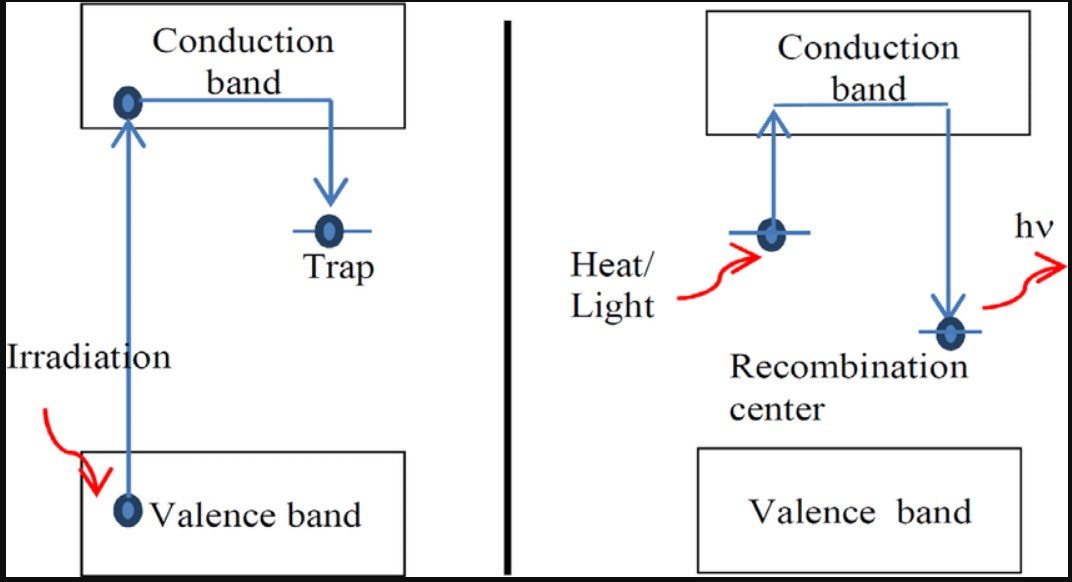
\includegraphics[width=0.5\textwidth]{Imagens/tldOsld.jpg}
			\caption{Exemplo da teoria de bandas nos fenômenos de termoluminescência (TLD - Aquecimento) e luminescência Opticamente estimulada (OSLD - Luz)}
			\label{}
		\end{figure}

	\section{Dosímetros Luminescentes Opticamente Estimulados (OSLD)}

		Os dosímetros OSLD (Optically Stimulated Luminescence Dosimeters) funcionam com base no fenômeno da luminescência estimulada opticamente. 

		Quando o dosímetro é exposto à radiação ionizante, ocorre a interação entre a radiação e os átomos do cristal, gerando íons e elétrons livres. Alguns dos elétrons livres ficam presos nas armadilhas eletrônicas do material sensível à radiação. Após a exposição à radiação, o dosímetro é colocado em um leitor de OSLD. Durante a leitura, o dosímetro é iluminado com uma luz de estimulação, geralmente na faixa de comprimento de onda ultravioleta ou visível. A luz de estimulação libera os elétrons presos nas armadilhas eletrônicas, fazendo com que retornem aos seus estados de energia mais baixos. À medida que os elétrons retornam aos seus estados de energia mais baixos, eles emitem luz na forma de luminescência. Essa luminescência é medida pelo leitor de OSLD, que converte o sinal óptico em um sinal elétrico proporcional à dose de radiação recebida pelo dosímetro. A intensidade da luminescência é proporcional à quantidade de radiação absorvida pelo dosímetro. O leitor de OSLD registra essa intensidade luminescente e calcula a dose de radiação com base em calibrações prévias, que relacionam a intensidade luminescente com a dose de radiação. A tecnologia OSLD é usada em serviços de dosimetria de radiações ionizantes por raios-x, gama e beta. Também pode ser empregada para detecção de nêutrons, embora este uso não seja praticado ainda no Brasil.

		Os principais materiais utilizados nos dosímetros OSL são:
		\begin{itemize}[label=\textcolor{CarnationPink}{$\star$}]
			\item \textbf{\ce{Al2O3}:\ce{C}} (Óxido de Alumínio dopado com Carbono): Emite uma luminescencia de 420 nm quando é estimulado com uma luz de 540 nm.
			\item \textbf{\ce{Al2O3}:\ce{C}, \ce{Mg}} (Óxido de Alumíno dopado com Carbono e Magnésio)
			\item O \textbf{\ce{Al2O3}} também pode ser dopado com elementos terras raras como o \ce{Ce} (cério) e o \ce{Tl} (tálio).
		\end{itemize}

		As principais \textcolor{CarnationPink}{VANTAGENS} em utilizar dosímetros OSL são:

		\begin{itemize}[label=\textcolor{CarnationPink}{$\blacktriangleright$}]
			\item \textbf{Alta sensibilidade:} Os dosímetros OSL são altamente sensíveis à radiação ionizante, permitindo a detecção e medição precisa de doses de radiação relativamente baixas. Isso é especialmente importante em áreas onde doses baixas são relevantes, como medicina nuclear e dose espalhada em radioterapia.
			\item \textbf{Ampla faixa de dose absorvida:} Os dosímetros OSL podem cobrir uma ampla faixa de dose de radiação, desde doses muito baixas até doses muito altas. Isso os torna adequados para diferentes aplicações, desde monitoramento de exposição ocupacional até medição de doses terapêuticas em radioterapia.
			\item \textbf{Estabilidade a longo prazo:} Os dosímetros OSL têm uma estabilidade a longo prazo em relação à resposta luminosa. Isso significa que eles mantêm sua calibração e resposta ao longo do tempo, o que é essencial para garantir medições confiáveis e consistentes ao longo de períodos prolongados.
			\item \textbf{Reutilização:} Os dosímetros OSL podem ser reutilizados após a leitura, o que os torna econômicos e sustentáveis. Após a leitura, a energia armazenada é liberada, permitindo que o dosímetro seja apagado e reutilizado para futuras medições, reduzindo custos.
			\item \textbf{Leitura rápida e eficiente:} A leitura dos dosímetros OSL é rápida e eficiente. Os dosímetros podem ser lidos em um leitor de OSL em poucos minutos, proporcionando resultados imediatos. Isso é particularmente útil em ambientes de saúde, onde é necessário monitorar rapidamente a exposição à radiação de pacientes e trabalhadores.
		\end{itemize}

		As principais \textcolor{CarnationPink}{DESVANTAGENS} em utilizar dosímetros OSL são:

		\begin{itemize}[label=\textcolor{CarnationPink}{$\blacktriangleright$}]
			\item \textbf{Sensibilidade à luz ambiente:} Os dosímetros OSL podem ser sensíveis à luz ambiente. Isso significa que a exposição à luz antes da leitura pode afetar a resposta do dosímetro, levando a resultados imprecisos. Portanto, é necessário tomar precauções para proteger o dosímetro da luz não intencional.
			\item \textbf{Complexidade da leitura:} A leitura dos dosímetros OSL requer equipamentos específicos, como leitores de OSL, que nem sempre estão disponíveis em todos os locais. Isso pode limitar a capacidade de leitura imediata em algumas situações e exigir a transferência dos dosímetros para um local apropriado para a leitura.
			\item \textbf{Sensibilidade a altas temperaturas:} Os dosímetros OSL podem ser sensíveis a altas temperaturas. Exposição a temperaturas elevadas pode levar a alterações na resposta do dosímetro e afetar a precisão das medições. É importante armazenar e manusear os dosímetros dentro dos limites de temperatura recomendados pelo fabricante.
			\item \textbf{Calibração específica:} Cada tipo de dosímetro OSL requer uma calibração específica para correlacionar a resposta luminosa com a dose de radiação. Isso implica que os dosímetros devem ser calibrados com uma fonte conhecida de radiação para cada tipo de aplicação específica. A falta de calibração adequada pode levar a medições imprecisas.
			\item \textbf{Dependência com o tipo de radiação:} A resposta dos dosímetros OSL pode variar dependendo do tipo de radiação ionizante. Eles podem ter diferentes eficiências de detecção para diferentes tipos de partículas (como fótons, elétrons ou nêutrons). Portanto, a resposta do dosímetro OSL pode não ser igual para todos os tipos de radiação, exigindo fatores de correção ou ajustes para diferentes tipos de exposição.
		\end{itemize}
		
		Uma característica dos OSLDs é a possibilidade de arquivamento do dosímetro e a verificação da dose por meio de leitura não-destrutiva, o que torna possível a reanálise completa das amostras e a realização de avaliações incrementais para rastreamento da exposição ao longo do tempo.
 
	\section{Calorímetros}

		O calorímetro utilizado para a dosimetria das radiações é um dispositivo projetado para medir a quantidade de energia térmica liberada quando a radiação ionizante interage com um material sensível. O princípio básico de funcionamento de um calorímetro é a conversão da energia depositada pela radiação em calor e a medição desse calor gerado, uma vez que a variação da temperatura na água devido a 1 Gy de dose absorvida é:
		
			\begin{equation}
				1 \; Gy = 2.4 \times 10^{-4}\;{}^{\circ}C \; na \; agua
			\end{equation}

		A determinação da dose absorvida através de um calorímetro se dá da seguinte forma:

		\begin{enumerate}
			\item \textbf{Material sensível:} O calorímetro é construído com um material sensível à radiação que tem a capacidade de converter a energia depositada pela radiação em calor de forma eficiente. Esse material pode ser um cristal, um líquido ou um polímero termossensível.
			\item \textbf{Calorimetria adiabática:} O calorímetro é projetado para ser termicamente isolado do ambiente externo, de forma que não haja troca significativa de calor com o ambiente durante a medida. Isso é chamado de calorimetria adiabática.
			\item \textbf{Absorção de energia:} Quando a radiação ionizante interage com o material sensível, ela deposita energia nesse material causando excitações ou ionizações que eventualmente levam os elétrons a se moverem para camadas mais altas, o que faz com que as moléculas vibrem mais rapidamente, que é basicamente o conceito por trás do calor. De fato, toda a radiação absorvida eventualmente aparece como calor e, portanto, isso pode ser medido com uma precisão muito alta em teoria.
			\item \textbf{Medida da temperatura:} A temperatura do calorímetro é medida utilizando sensores de temperatura sensíveis e precisos. Esses sensores podem ser termopares, termorresistências (RTDs) ou termistores.
			\item \textbf{Calibração:} O calorímetro deve ser calibrado previamente usando fontes de radiação de referência para estabelecer uma relação entre a quantidade de calor gerado e a dose de radiação absorvida.
			\item \textbf{Cálculo da dose}: Com base na medição da temperatura e nas características do calorímetro, é possível calcular a dose de radiação absorvida pelo material sensível, com base nos parâmetros prévios de calibração. 
		\end{enumerate}

		Os calorímetros utilizados na dosimetria de radiação fornecem uma medida direta da quantidade de energia depositada pela radiação, permitindo uma determinação precisa da dose absorvida. No entanto, eles requerem uma calibração cuidadosa e podem ser mais complexos em comparação com outros métodos de dosimetria de radiação, como os TLDs ou os OSLDs, pois a variação de temperatura é muito pequena, necessitando de um equipamento com uma precisão muito alta, e, portanto, não é considerado muito prático.

	\section{Filmes Radiográficos}

		Os filmes radiográficos são utilizados tanto para fins de diagnóstico em radiologia como para dosimetria das radiações. A sua utilização na dosimetria envolve o princípio da interação da radiação ionizante com a emulsão fotossensível presente no filme.

		Os filmes são constituídos e são utilizados na dosimetria das radiações da seguinte forma:

		\begin{itemize}
			\item \textbf{Estrutura do filme:} Os filmes radiográficos são compostos por uma emulsão fotossensível, geralmente à base de prata, que é sensível à radiação ionizante. A emulsão contém grãos de brometo de prata halogenada dispersos em uma matriz gelatinosa.
			\item \textbf{Interação com a radiação:} Quando a radiação ionizante, como raios-X ou raios gama, incide no filme, ocorre uma interação com os grãos de prata halogenada. Essa interação resulta na ionização e excitação dos átomos da prata presentes nos grãos.
			\item \textbf{Formação da Imagem Latente:} A ionização e excitação dos átomos na emulsão fotossensível causam uma modificação estrutural nos grãos de prata halogenada (reação química), formando uma imagem latente. Essa imagem latente não é visível a olho nu.
			\item \textbf{Processamento do filme:} O filme é submetido a um processo químico chamado de revelação, fixação e lavagem para revelar a imagem latente. A revelação envolve a redução dos grãos de prata ionizados a grãos metálicos de prata, enquanto a fixação remove os grãos não expostos. A lavagem final remove os resíduos químicos do processo.
			\item \textbf{Leitura da imagem:} Após o processamento, a imagem resultante no filme radiográfico é visualizada. A densidade e a distribuição dos grãos de prata revelados refletem a quantidade de radiação absorvida pelo filme durante a exposição, onde a quantidade de radiação corresponde à quantidade de prata restante e, portanto, ao escurecimento.
		\end{itemize}

		As principais \textcolor{CarnationPink}{VANTAGENS} na utilização de Filmes Radiográficos são:

		\begin{itemize}[label=\textcolor{CarnationPink}{$\blacktriangleright$}]
			\item \textbf{Amplamente disponíveis:} Os filmes radiográficos são amplamente utilizados na prática clínica e estão disponíveis em muitos centros de saúde e hospitais. Isso facilita o acesso a esses materiais para a dosimetria das radiações.
			\item \textbf{Baixo custo}: Os filmes radiográficos são relativamente baratos em comparação com outros sistemas de dosimetria mais avançados. Isso os torna uma opção acessível, especialmente em conções com recursos limitados.
			\item \textbf{Registro permanente:} Os filmes radiográficos fornecem um registro permanente da imagem e da distribuição de dose, permitindo uma documentação precisa dos resultados da dosimetria.
			\item \textbf{Alta resolução espacial:} Os filmes radiográficos têm alta resolução espacial. A resolução espacial obtida por filmes radiográficos refere-se à capacidade do filme em capturar e reproduzir detalhes espaciais finos na imagem radiográfica. É uma medida da capacidade do filme em distinguir estruturas pequenas e próximas umas das outras; O que significa que eles podem fornecer detalhes precisos sobre a distribuição da dose em uma região específica. Ou seja, feixes de elétrons e feixes de fótons de megavoltagem podem ter suas isodoses medidas com relativa precisão e principalmente a forma de um feixe pode ser determinada.
			\item \textbf{Sensibilidade à radiação:} Os filmes radiográficos têm uma resposta sensível à radiação ionizante, o que os torna úteis para medir uma ampla faixa de radiação.
		\end{itemize}

		As principais \textcolor{CarnationPink}{DESVANTAGENS} na utilização de filmes radiográficos são:

		\begin{itemize}[label=\textcolor{CarnationPink}{$\blacktriangleright$}]
			\item \textbf{Processamento químico}: Os filmes radiográficos requerem processamento químico para revelar a imagem latente, o que pode ser demorado e exigir instalações específicas.
			\item \textbf{Resposta não linear:} Os filmes radiográficos têm uma resposta não linear à radiação, o que significa que a densidade óptica dos grãos revelados pode não ser diretamente proporcional à dose absorvida. Isso requer uma calibração cuidadosa para obter resultados precisos.
			\item \textbf{Efeito de sobreposição:} Quando múltiplos filmes são utilizados em conjunto para medir distribuições de dose complexas, pode haver sobreposição entre as imagens, dificultando a interpretação precisa dos resultados.
			\item \textbf{Limitações de tempo e temperatura:} Os filmes radiográficos podem ser sensíveis ao tempo e à temperatura, o que pode afetar a estabilidade e a precisão das medições. O armazenamento e a manipulação adequadas são essenciais para garantir resultados confiáveis, além disso os filmes são sensíveis à luz visível, podendo ser contaminados.
			\item \textbf{Dificuldade na automação e análise:} A análise dos filmes radiográficos geralmente requer um processo manual, o que pode ser demorado e sujeito a erros. Além disso, a automação e a análise objetiva podem ser desafiadoras devido à natureza analógica dos filmes.
		\end{itemize}

	\section{Filmes Radiocrômicos}

		O filme radiocrômico é um tipo especial de filme que muda de cor quando exposto à radiação ionizante. Diferente dos filmes radiográficos convencionais, que são sensíveis à luz, os filmes radiocrômicos não são sensíveis à luz visível (embora ainda seja sensível à luz UV).

		A composição dos filmes radiocrômicos pode variar dependendo do fabricante, mas geralmente eles são compostos por uma matriz polimérica contendo um material sensibilizador. O material sensibilizador é responsável por reagir com a radiação ionizante e causar uma mudança na cor do filme. Quando o filme radiocrômico é exposto à radiação ionizante, ocorrem interações entre os raios X, raios gama ou outras partículas da radiação e o material sensibilizador. Essas interações podem resultar em danos na estrutura molecular do material sensibilizador, que por sua vez causam mudanças na absorção ou reflexão da luz pelo filme. A mudança na absorção ou reflexão da luz afeta a cor percebida do filme. A quantidade de radiação absorvida determinará a magnitude da mudança de cor. Através da análise dessa mudança de cor, é possível determinar a dose de radiação absorvida pelo filme.

		Portanto, o processo de dosimetria utilizando filmes radiocrômicos ocorre da seguinte maneira:
		\begin{enumerate}
			\item \textbf{Exposição à radiação:} O filme radiocrômico é colocado em uma região onde a radiação ionizante será medida. A radiação interage com o material sensibilizador no filme, causando danos ou modificando a estrutura molecular do material.
			\item Mudança de cor: A interação da radiação provoca uma mudança na cor do filme. A magnitude da mudança de cor está relacionada à quantidade de radiação absorvida pelo filme.
			\item \textbf{Análise da mudança de cor:} Após a exposição, o filme radiocrômico é analisado para determinar a mudança de cor. Isso pode ser feito visualmente, comparando a cor do filme antes e depois da exposição, ou por meio de equipamentos específicos que medem a absorção de luz em diferentes comprimentos de onda.
			\item \textbf{Calibração:} Antes do uso do filme radiocrômico como dosímetro, é necessário realizar uma calibração. Isso envolve a exposição do filme a uma série conhecida de doses de radiação e a correlação entre a mudança de cor e a dose absorvida é estabelecida.
			\item \textbf{Interpretação da dose:} Com base na mudança de cor medida no filme radiocrômico, é possível determinar a dose de radiação absorvida pelo filme. A relação entre a mudança de cor e a dose é utilizada para fazer essa determinação.
		\end{enumerate}

		
		As principais \textcolor{CarnationPink}{VANTAGENS} na utilização de filmes radiocrômicos são:

		\begin{itemize}[label=\textcolor{CarnationPink}{$\blacktriangleright$}]
			\item \textbf{Alta resolução espacial:} Os filmes radiocrômicos possuem alta resolução espacial, o que significa que eles podem fornecer informações detalhadas sobre a distribuição espacial da dose de radiação. Isso é especialmente útil em aplicações onde é necessário mapear a distribuição precisa da dose em uma área específica.
			\item \textbf{Sensibilidade a diferentes tipos de radiação:} Os filmes radiocrômicos podem ser sensíveis a uma ampla gama de radiações ionizantes, incluindo raios X, raios gama, partículas alfa, partículas beta, entre outras. Isso os torna versáteis em termos de aplicação, permitindo a dosimetria de diferentes tipos de radiação.
			\item \textbf{Não requer fonte de energia externa:} Os filmes radiocrômicos não exigem fonte de energia externa para funcionar. Eles são passivos e não necessitam de eletricidade ou baterias, tornando-os convenientes para uso em diferentes conções e ambientes.
		\end{itemize}

		As principais \textcolor{CarnationPink}{DESVANTAGENS} em utilizar filmes radiocrômicos são:

		\begin{itemize}[label=\textcolor{CarnationPink}{$\blacktriangleright$}]
			\item \textbf{Calibração e interpretação complexas:} A calibração dos filmes radiocrômicos requer procedimentos cuidadosos para correlacionar a mudança de cor com a dose de radiação absorvida. Além disso, a interpretação dos resultados também pode ser complexa, exigindo equipamentos específicos e experiência adequada.
			\item \textbf{Leitura subjetiva:} A leitura e interpretação da mudança de cor dos filmes radiocrômicos podem ser subjetivas, dependendo da percepção visual do observador. Isso pode introduzir certa subjetividade nas medições e afetar a precisão dos resultados.
			\item \textbf{Limitações de faixa de dose:} Os filmes radiocrômicos podem ter limitações em termos de faixa de dose que podem ser medidos com precisão. Cada tipo de filme radiocrômico tem sua própria faixa de dose linear e acima ou abaixo dessa faixa, a resposta pode não ser linear ou pode ocorrer saturação.
			\item \textbf{Limitação de tempo de resposta:} Os filmes radiocrômicos podem ter um tempo de resposta relativamente lento para desenvolver completamente a mudança de cor após a exposição à radiação. Dependendo do tipo de filme e das condições de processamento, pode levar horas, para que a mudança de cor se estabilize completamente. Essa limitação de tempo de resposta pode ser inconveniente em situações onde a resposta imediata é necessária, especialmente em ambientes de monitoramento em tempo real ou em casos de acidentes radiológicos.
		\end{itemize}


	\section{Dosímetro de Fricke}

		O dosímetro de Fricke é um tipo de dosímetro químico utilizado para medir a dose absorvida de radiação . Ele é baseado na propriedade do sal de Fricke, uma solução de sulfato ferroso  em ácido sulfúrico (\ce{H2SO4}), de sofrer uma mudança de cor devido aos íons férricos formados quando exposto à radiação ionizante.

		O processo de funcionamento do dosímetro de Fricke se dá pela seguinte maneira:

		\begin{enumerate}
			\item \textbf{Preparação do dosímetro:} Uma solução de sal de Fricke é preparada cuidadosamente em laboratório, utilizando sulfato ferroso, cloreto de sódio, ácido sulfúrico e água. A concentração da solução é ajustada para fornecer uma resposta linear à radiação dentro da faixa de dose de radiação avaliada. Normalmente é utilizado uma concentração de 1 mmol/L de sulfato ferroso, 1 mmol/L de \ce{NaCl} e 0,4 mol/L de \ce{H2SO4}.
			\item \textbf{Exposição à radiação:} O dosímetro de Fricke é exposto à radiação ionizante que se deseja medir a dose absorvida. A radiação interage com os íons da solução de Fricke, causando uma série de reações químicas;
			\item \textbf{Formação de íons férricos:} A radiação ionizante converte os íons ferrosos (\ce{Fe^2+}) em íons férricos (\ce{Fe^3+}). Essa conversão ocorre devido à oxidação do ferro induzida pelo processo de ionização.
			\item \textbf{Mudança de cor:} Os íons férricos (\ce{Fe^3+}) formados na solução de Fricke têm uma coloração diferente dos íons ferrosos (\ce{Fe^2+}). A mudança de cor é geralmente uma mudança do tom verde para o tom azul.
			\item \textbf{Medição da absorção de radiação:} A magnitude da mudança de cor (concentração de íons férricos) é proporcional à quantidade de radiação absorvida pela solução de Fricke. Essa concentração de íons férricos pode ser quantificada por meio de técnicas espectrofotométricas, que medem a absorção de luz em uma determinada faixa de comprimento de onda. (Picos de absorção UV em 224 nm e 304 nm).
			\item \textbf{Cálculo da dose de radiação absorvida:} A magnitude da mudança de cor é relacionada a uma dose de radiação específica por meio de uma curva de calibração pré-determinada. Com base nessa curva, é possível determinar a dose de radiação absorvida pelo dosímetro de Fricke.
		\end{enumerate}

		Infelizmente, nem todas as energias dos fótons criam o mesmo número de reações, então existem tabelas de “valores G” que são o número de moléculas produzidas por 100 eV de energia absorvida. O número é de cerca de 15,5 moléculas por 100 eV absorvidos e esse valor de G não muda muito para energias usadas em radiação oncológica.

		O dosímetro de Fricke é um método amplamente utilizado em pesquisas em radioterapia, permitindo uma medição precisa da dose de radiação absorvida. No entanto, requer preparação cuidadosa da solução de Fricke, calibração adequada e análise precisa da concentração de íons férricos para obter resultados confiáveis.

	\section{Detectores de Estado Sólido (Diodos Semicondutores)}

	Os detectores de radiação de estado sólido, também conhecidos como diodos detectores de radiação, são dispositivos semicondutores que são sensíveis à radiação ionizante. Eles são amplamente utilizados para detectar e medir a radiação em diversas aplicações, como medicina nuclear, radioterapia, monitoramento ambiental e segurança nuclear.

	Os detectores semicondutores funcionam da seguinte maneira:

		\begin{enumerate}
			\item \textbf{Material semicondutor:} O detector de radiação de estado sólido é feito de um material semicondutor, como o silício ou o germânio. Esses materiais possuem propriedades eletrônicas específicas que os tornam sensíveis à radiação ionizante.
			\item \textbf{Estrutura de diodo:} O detector é projetado na forma de um diodo semicondutor, que é basicamente uma junção p-n entre duas regiões com diferentes tipos de dopagem. Essa estrutura cria uma região de depleção, onde não há portadores de carga livres.
			\item \textbf{Interação com a radiação:} Quando a radiação ionizante atinge o material semicondutor, ela interage com os átomos do material e produz pares elétrons-buracos. Esses pares elétrons-buracos são criados por processos como ionização e excitação eletrônica.
			\item \textbf{Geração de carga:} Os pares de elétrons-buracos gerados pela radiação se movem na região de depleção do diodo. Os elétrons são capturados pela região n, enquanto os buracos são capturados pela região p. Esse movimento de cargas gera um sinal elétrico proporcional à quantidade de radiação absorvida.
			\item \textbf{Coleta e amplificação do sinal:} O sinal elétrico gerado pelos pares elétrons-buracos é coletado pelos contatos metálicos do diodo e direcionado para um circuito de leitura. Nesse circuito, o sinal é amplificado e processado para análise e medição.
			\item \textbf{Detecção e quantificação da radiação:} Com base no sinal elétrico amplificado e processado, é possível detectar e quantificar a radiação absorvida pelo detector de estado sólido. A magnitude do sinal está diretamente relacionada à energia e à intensidade da radiação.
		\end{enumerate}
		
		Os principais materiais utilizados em um semicondutor são:

			\begin{itemize}[label=\textcolor{CarnationPink}{$\star$}]
				\item \textbf{Silício (Si):} O silício é o material semicondutor mais amplamente utilizado na indústria eletrônica. É abundante, possui um intervalo de energia adequado e pode ser facilmente dopado para criar diodos com diferentes características. É bastante sensível à radiação ionizante, especialmente para detectar radiação de partículas alfa. O silício pode ser dopado com átomos de fósforo (P) para criar o semicondutor tipo n adicionando elétrons extras, ou com átomos de boro (B) para criar o semicondutor tipo p, adicionando buracos.
				
				\item \textbf{Germânio (Ge):} O germânio é um material semicondutor que apresenta maior eficiência na detecção de radiação ionizante em comparação ao silício. É frequentemente usado em detectores de radiação de alta energia, como a espectrometria de raios X.  O germânio pode ser dopado de maneira semelhante ao silício, utilizando átomos de fósforo para criar o tipo n e átomos de boro para criar o tipo p.
				
				\item \textbf{Telureto de cádmio (CdTe):} O telureto de cádmio é um material semicondutor composto usado em detectores de radiação de alta eficiência, especialmente para detecção de raios X e gama. É dopado com impurezas de cádmio (Cd) e telúrio (Te) para ajustar suas propriedades elétricas.

				\item \textbf{Telureto de cádmio-zinco (CdZnTe):} O CdZnTe é outro material semicondutor composto usado em detectores de radiação, especialmente para aplicações de detecção de raios X e gama. Ele é dopado com impurezas de cádmio (Cd) e zinco (Zn).
			\end{itemize}

			Algumas \textcolor{CarnationPink}{VANTAGENS} em utilizar detectores de diodos são:

			\begin{itemize}[label=\textcolor{CarnationPink}{$\blacktriangleright$}]
				\item \textbf{Alta sensibilidade:} Os diodos semicondutores têm uma alta sensibilidade à radiação ionizante, permitindo a detecção de níveis muito baixos de radiação.
				\item \textbf{Resposta rápida:} Os diodos semicondutores têm uma resposta rápida à radiação, permitindo uma medição em tempo real da dose de radiação.
				\item \textbf{Faixa dinâmica ampla:} Os diodos semicondutores possuem uma ampla faixa dinâmica, o que significa que podem medir uma ampla gama de doses de radiação, desde níveis baixos até níveis muito altos.
				\item \textbf{Tamanho compacto:} Os diodos semicondutores são dispositivos pequenos e compactos, o que facilita sua integração em sistemas e equipamentos de detecção.
			\end{itemize}

			Algumas \textcolor{CarnationPink}{DESVANTAGENS} em utilizar diodos são:

			\begin{itemize}[label=\textcolor{CarnationPink}{$\blacktriangleright$}]
				\item \textbf{Sensibilidade à temperatura:} Os diodos semicondutores são sensíveis a variações de temperatura, o que pode afetar sua resposta e precisão na medição da dose de radiação.
				\item \textbf{Efeito de dano por radiação:} A exposição prolongada à radiação pode causar danos ao material do diodo, levando a alterações em suas propriedades elétricas e, eventualmente, à falha do dispositivo.
				\item \textbf{Custo}: Os diodos semicondutores, especialmente aqueles de alta qualidade e desempenho, podem ser relativamente caros em comparação com outros tipos de detectores de radiação.
				\item \textbf{Efeito de envelhecimento:} Com o tempo, os diodos semicondutores podem sofrer degradação de desempenho devido ao envelhecimento, o que pode levar a uma diminuição da sensibilidade e precisão ao longo do tempo.
				\item \textbf{Efeito da Geometria:} Este detector tem variabilidade no posicionamento causando uma dependência direcional, possui dependência energética em feixes de fótons,
			\end{itemize}
		
	\section{Detectores MOSFET}

		Os detectores MOSFETs (Metal-Oxide-Semiconductor Field-Effect Transistors) são dispositivos semicondutores que são amplamente utilizados como detectores de radiação. Eles são baseados na tecnologia dos transistores de efeito de campo (FET) de óxido de metal-semicondutor (MOS).

		Os detectores MOSFET consistem em uma estrutura de três camadas: o substrato semicondutor, o óxido de isolamento e o metal de controle. O substrato semicondutor é dopado para criar uma região tipo p (p-channel MOSFET) ou tipo n (n-channel MOSFET). O óxido de isolamento é depositado sobre o substrato e atua como um isolante elétrico. O metal de controle é aplicado sobre o óxido de isolamento e funciona como o terminal de controle do transistor.
	
		Quando um MOSFET é irradiado com radiação ionizante, a interação da radiação com o substrato semicondutor gera pares de elétrons e buracos. Esses portadores de carga afetam a condutividade do substrato semicondutor, resultando em uma alteração na corrente elétrica que flui através do MOSFET. Essa alteração na corrente é proporcional à dose de radiação incidente.
	
		Os detectores MOSFET possuem várias vantagens, como alta sensibilidade, resposta rápida, faixa dinâmica ampla, boa resolução espacial e baixo consumo de energia. Além disso, eles são reutilizáveis e podem ser facilmente integrados a sistemas de leitura e análise.

	\section{Cintiladores}

		Os detectores de cintilação, também conhecidos como detectores de cintiladores, são dispositivos que convertem a energia da radiação incidente em luz visível ou infravermelha próxima. Essa conversão ocorre dentro de um material chamado cintilador, que é composto por cristais ou materiais orgânicos.

		Quando a radiação ionizante interage com o cintilador, ela transfere parte de sua energia para os átomos ou moléculas do material. Essa energia é absorvida pelos elétrons do cintilador, que são promovidos para estados de energia mais elevados. Em seguida, esses elétrons retornam aos seus estados fundamentais, liberando a energia excessiva na forma de fótons de luz.
	
		Os fótons de luz emitidos durante o processo de cintilação podem ser detectados por um fotodetector, como um fotomultiplicador (PMT) ou um fotodiodo. O fotodetector converte os fótons de luz em sinais elétricos, que podem ser amplificados e registrados para análise posterior.

		Os detectores de cintilação são utilizados em uma ampla variedade de aplicações de detecção de radiação, incluindo medicina nuclear, detecção de partículas, espectroscopia de raios-X, radiografia industrial e detecção de radiação cósmica. Eles são especialmente úteis quando é necessário distinguir diferentes tipos de radiação ou medir a energia dos fótons incidentes.
			
		Os principais detectores cintiladores são:

		\begin{itemize}[label=\textcolor{CarnationPink}{$\star$}]
			\item \textbf{\ce{NaI}} (Iodeto de Sódio): É um cintilador inorgânico amplamente utilizado em detecção de radiação gama e detecção de raios-X.
			\item \textbf{\ce{Na(Tl)}} (Iodeto de Sódio dopado com tálio): é uma forma do \ce{NaI} dopado com tálio para aumentar sua eficiência de cintilação.
			\item \textbf{\ce{CsI}} (Iodeto de Césio): sim como o iodeto de sódio, o CsI é um cintilador inorgânico utilizado na detecção de radiação gama e raios-X. É conhecido por sua boa resolução energética.
			\item \textbf{\ce{Gd2O3}} (Óxido de Gadolínio): É um cintilador inorgânico usado principalmente em detecção de nêutrons térmicos. Ele possui uma alta eficiência de cintilação para radiação de nêutrons e é frequentemente combinado com materiais conversores para detectar a radiação resultante da interação dos nêutrons.
			\item \textbf{\ce{C14H10}} (Antraceno): É um cintilador orgânico utilizado principalmente na detecção de radiação alfa. É sensível a partículas carregadas de alta energia e é frequentemente utilizado em detectores de partículas.
		\end{itemize}
	
		As principais \textcolor{CarnationPink}{VANTAGENS} em utilizar cintiladores :

		\begin{itemize}[label=\textcolor{CarnationPink}{$\blacktriangleright$}]
			\item \textbf{Alta eficiência de detecção:} Os detectores cintiladores podem ter uma alta eficiência de detecção para uma ampla faixa de energias de radiação, o que permite a detecção de baixas doses de radiação.
			\item \textbf{Alta sensibilidade:} Os cintiladores podem ser altamente sensíveis à radiação, permitindo a detecção de até mesmo pequenas quantidades de radiação.
			\item \textbf{Boa resolução energética:} Alguns cintiladores possuem uma boa resolução energética, o que significa que eles podem distinguir diferentes níveis de energia da radiação incidente.
			\item \textbf{Versatilidade:} Existem diversos tipos de cintiladores disponíveis, cada um adequado para diferentes tipos de radiação e aplicações específicas, o que torna os detectores cintiladores versáteis.
		\end{itemize}

		As principais \textcolor{CarnationPink}{DESVANTAGENS}  em utilizar cintiladores:

		\begin{itemize}[label=\textcolor{CarnationPink}{$\blacktriangleright$}]
			\item \textbf{Decaimento temporal:} Alguns cintiladores podem apresentar um decaimento temporal prolongado, o que pode levar a uma resposta lenta do detector e afetar a precisão temporal das medidas.
			\item \textbf{Sensibilidade à temperatura:} Alguns cintiladores são sensíveis à temperatura, o que pode afetar a resposta do detector e requerer medidas de controle de temperatura.
			\item \textbf{Efeito de saturação:} Em altas intensidades de radiação, os detectores cintiladores podem atingir uma saturação, o que pode limitar sua capacidade de medir doses muito altas.
			\item \textbf{Fragilidade:} Alguns cintiladores são frágeis e ser danificados facilmente, exigindo manuseio cuidadoso e proteção adequada.			
			\item \textbf{Influência da luz ambiente:} A presença de luz ambiente pode interferir na medição dos cintiladores, exigindo medidas de controle de luz adequadas.
		\end{itemize}

		



\bibliography{ref.bib}
\end{document}